\documentclass{article}

\usepackage{arxiv}

\usepackage[utf8]{inputenc} % allow utf-8 input
\usepackage[T1]{fontenc}    % use 8-bit T1 fonts
\usepackage{lmodern}        % https://github.com/rstudio/rticles/issues/343
\usepackage{hyperref}       % hyperlinks
\usepackage{url}            % simple URL typesetting
\usepackage{booktabs}       % professional-quality tables
\usepackage{amsfonts}       % blackboard math symbols
\usepackage{nicefrac}       % compact symbols for 1/2, etc.
\usepackage{microtype}      % microtypography
\usepackage{graphicx}

\title{Reference Solutions}

\author{
    Taojun Hu
    \thanks{If you find any errors including typos, it's welcomed to
contact me by email}
   \\
    Department of Biostatistics \\
    Peking University \\
   \\
  \texttt{\href{mailto:2011110158@stu.pku.edu.cn}{\nolinkurl{2011110158@stu.pku.edu.cn}}} \\
  }

\usepackage{color}
\usepackage{fancyvrb}
\newcommand{\VerbBar}{|}
\newcommand{\VERB}{\Verb[commandchars=\\\{\}]}
\DefineVerbatimEnvironment{Highlighting}{Verbatim}{commandchars=\\\{\}}
% Add ',fontsize=\small' for more characters per line
\usepackage{framed}
\definecolor{shadecolor}{RGB}{248,248,248}
\newenvironment{Shaded}{\begin{snugshade}}{\end{snugshade}}
\newcommand{\AlertTok}[1]{\textcolor[rgb]{0.94,0.16,0.16}{#1}}
\newcommand{\AnnotationTok}[1]{\textcolor[rgb]{0.56,0.35,0.01}{\textbf{\textit{#1}}}}
\newcommand{\AttributeTok}[1]{\textcolor[rgb]{0.77,0.63,0.00}{#1}}
\newcommand{\BaseNTok}[1]{\textcolor[rgb]{0.00,0.00,0.81}{#1}}
\newcommand{\BuiltInTok}[1]{#1}
\newcommand{\CharTok}[1]{\textcolor[rgb]{0.31,0.60,0.02}{#1}}
\newcommand{\CommentTok}[1]{\textcolor[rgb]{0.56,0.35,0.01}{\textit{#1}}}
\newcommand{\CommentVarTok}[1]{\textcolor[rgb]{0.56,0.35,0.01}{\textbf{\textit{#1}}}}
\newcommand{\ConstantTok}[1]{\textcolor[rgb]{0.00,0.00,0.00}{#1}}
\newcommand{\ControlFlowTok}[1]{\textcolor[rgb]{0.13,0.29,0.53}{\textbf{#1}}}
\newcommand{\DataTypeTok}[1]{\textcolor[rgb]{0.13,0.29,0.53}{#1}}
\newcommand{\DecValTok}[1]{\textcolor[rgb]{0.00,0.00,0.81}{#1}}
\newcommand{\DocumentationTok}[1]{\textcolor[rgb]{0.56,0.35,0.01}{\textbf{\textit{#1}}}}
\newcommand{\ErrorTok}[1]{\textcolor[rgb]{0.64,0.00,0.00}{\textbf{#1}}}
\newcommand{\ExtensionTok}[1]{#1}
\newcommand{\FloatTok}[1]{\textcolor[rgb]{0.00,0.00,0.81}{#1}}
\newcommand{\FunctionTok}[1]{\textcolor[rgb]{0.00,0.00,0.00}{#1}}
\newcommand{\ImportTok}[1]{#1}
\newcommand{\InformationTok}[1]{\textcolor[rgb]{0.56,0.35,0.01}{\textbf{\textit{#1}}}}
\newcommand{\KeywordTok}[1]{\textcolor[rgb]{0.13,0.29,0.53}{\textbf{#1}}}
\newcommand{\NormalTok}[1]{#1}
\newcommand{\OperatorTok}[1]{\textcolor[rgb]{0.81,0.36,0.00}{\textbf{#1}}}
\newcommand{\OtherTok}[1]{\textcolor[rgb]{0.56,0.35,0.01}{#1}}
\newcommand{\PreprocessorTok}[1]{\textcolor[rgb]{0.56,0.35,0.01}{\textit{#1}}}
\newcommand{\RegionMarkerTok}[1]{#1}
\newcommand{\SpecialCharTok}[1]{\textcolor[rgb]{0.00,0.00,0.00}{#1}}
\newcommand{\SpecialStringTok}[1]{\textcolor[rgb]{0.31,0.60,0.02}{#1}}
\newcommand{\StringTok}[1]{\textcolor[rgb]{0.31,0.60,0.02}{#1}}
\newcommand{\VariableTok}[1]{\textcolor[rgb]{0.00,0.00,0.00}{#1}}
\newcommand{\VerbatimStringTok}[1]{\textcolor[rgb]{0.31,0.60,0.02}{#1}}
\newcommand{\WarningTok}[1]{\textcolor[rgb]{0.56,0.35,0.01}{\textbf{\textit{#1}}}}


% Pandoc citation processing

\usepackage{amsmath}
\usepackage{enumerate}


\begin{document}
\maketitle

\def\tightlist{}


\begin{abstract}

\end{abstract}


\hypertarget{homework}{%
\section{Homework}\label{homework}}

\begin{itemize}
\tightlist
\item
  chapter 2: page 244, 3(2); page 246 4; page 247 3(1) and page 248 4(1)
\item
  chapter 3: page 249 3(1)(2)(4)
\item
  chapter 4: page 254 3(3)(4); page 256 3(1)(4)
\item
  chapter 5: page 258 1; page 258 2, 3
\end{itemize}

\hypertarget{reference-solutions}{%
\section{Reference solutions}\label{reference-solutions}}

\begin{Shaded}
\begin{Highlighting}[]
\CommentTok{\# please first library the following packages: tidyverse, ggpubr}
\CommentTok{\# if (! require(pacman)) install.packages("pacman")}
\CommentTok{\# pacman::p\_load(tidyverse, ggpubr)}
\end{Highlighting}
\end{Shaded}

\hypertarget{solutions-for-chapter-2}{%
\subsection{Solutions for chapter 2}\label{solutions-for-chapter-2}}

\begin{enumerate}
\def\labelenumi{\arabic{enumi}.}
\tightlist
\item
  (Page 244 3(2))
\end{enumerate}

\begin{Shaded}
\begin{Highlighting}[]
\NormalTok{get.per }\OtherTok{\textless{}{-}} \ControlFlowTok{function}\NormalTok{(lower, upper)\{}
  \FunctionTok{pnorm}\NormalTok{(upper, }\AttributeTok{mean =} \DecValTok{146}\NormalTok{, }\AttributeTok{sd =} \DecValTok{8}\NormalTok{) }\SpecialCharTok{{-}} \FunctionTok{pnorm}\NormalTok{(lower, }\AttributeTok{mean =} \DecValTok{146}\NormalTok{, }\AttributeTok{sd =} \DecValTok{8}\NormalTok{)\}}
\FunctionTok{get.per}\NormalTok{(}\DecValTok{138}\NormalTok{, }\DecValTok{154}\NormalTok{)}
\end{Highlighting}
\end{Shaded}

\begin{verbatim}
## [1] 0.6826895
\end{verbatim}

\begin{Shaded}
\begin{Highlighting}[]
\FunctionTok{get.per}\NormalTok{(}\DecValTok{130}\NormalTok{, }\DecValTok{162}\NormalTok{)}
\end{Highlighting}
\end{Shaded}

\begin{verbatim}
## [1] 0.9544997
\end{verbatim}

\begin{enumerate}
\def\labelenumi{\arabic{enumi}.}
\setcounter{enumi}{1}
\tightlist
\item
  (Page 246 4)
\end{enumerate}

\begin{Shaded}
\begin{Highlighting}[]
\NormalTok{data.co }\OtherTok{\textless{}{-}} \FunctionTok{data.frame}\NormalTok{(}\AttributeTok{transfer =} \FunctionTok{c}\NormalTok{(}\StringTok{\textquotesingle{}no\textquotesingle{}}\NormalTok{, }\StringTok{\textquotesingle{}yes\textquotesingle{}}\NormalTok{), }\AttributeTok{a\_case =} \FunctionTok{c}\NormalTok{(}\DecValTok{45}\NormalTok{, }\DecValTok{710}\NormalTok{), }
                      \AttributeTok{a\_survive =} \FunctionTok{c}\NormalTok{(}\DecValTok{35}\NormalTok{, }\DecValTok{450}\NormalTok{), }\AttributeTok{b\_case =} \FunctionTok{c}\NormalTok{(}\DecValTok{300}\NormalTok{, }\DecValTok{83}\NormalTok{), }
                      \AttributeTok{b\_survive =} \FunctionTok{c}\NormalTok{(}\DecValTok{215}\NormalTok{, }\DecValTok{42}\NormalTok{)) }\SpecialCharTok{\%\textgreater{}\%}
    \FunctionTok{mutate}\NormalTok{(}\AttributeTok{a\_rate =}\NormalTok{ a\_survive}\SpecialCharTok{/}\NormalTok{a\_case, }\AttributeTok{b\_rate =}\NormalTok{ b\_survive}\SpecialCharTok{/}\NormalTok{b\_case) }\SpecialCharTok{\%\textgreater{}\%}
    \FunctionTok{mutate}\NormalTok{(}\AttributeTok{total =}\NormalTok{ a\_case }\SpecialCharTok{+}\NormalTok{ b\_case) }\SpecialCharTok{\%\textgreater{}\%}
    \FunctionTok{mutate}\NormalTok{(}\AttributeTok{a\_surv =}\NormalTok{ a\_rate}\SpecialCharTok{*}\NormalTok{total, }\AttributeTok{b\_surv =}\NormalTok{ b\_rate}\SpecialCharTok{*}\NormalTok{total)}

\NormalTok{data.simplify }\OtherTok{\textless{}{-}}\NormalTok{ data.co }\SpecialCharTok{\%\textgreater{}\%}\NormalTok{ dplyr}\SpecialCharTok{::}\FunctionTok{select}\NormalTok{(}\FunctionTok{c}\NormalTok{(}\StringTok{\textquotesingle{}total\textquotesingle{}}\NormalTok{, }\StringTok{\textquotesingle{}a\_surv\textquotesingle{}}\NormalTok{, }\StringTok{\textquotesingle{}b\_surv\textquotesingle{}}\NormalTok{)) }\SpecialCharTok{\%\textgreater{}\%}
    \FunctionTok{colSums}\NormalTok{()}
\NormalTok{a\_std\_surv }\OtherTok{=}\NormalTok{ data.simplify[}\DecValTok{2}\NormalTok{]}\SpecialCharTok{/}\NormalTok{data.simplify[}\DecValTok{1}\NormalTok{]}
\NormalTok{b\_std\_surv }\OtherTok{=}\NormalTok{ data.simplify[}\DecValTok{3}\NormalTok{]}\SpecialCharTok{/}\NormalTok{data.simplify[}\DecValTok{1}\NormalTok{]}
\FunctionTok{cat}\NormalTok{(}\StringTok{\textquotesingle{}Standard survival rate for hospital A: \textquotesingle{}}\NormalTok{, a\_std\_surv, }\StringTok{\textquotesingle{}}\SpecialCharTok{\textbackslash{}n}\StringTok{\textquotesingle{}}\NormalTok{)}
\end{Highlighting}
\end{Shaded}

\begin{verbatim}
## Standard survival rate for hospital A:  0.6774508
\end{verbatim}

\begin{Shaded}
\begin{Highlighting}[]
\FunctionTok{cat}\NormalTok{(}\StringTok{\textquotesingle{}Standard survival rate for hospital B: \textquotesingle{}}\NormalTok{, b\_std\_surv, }\StringTok{\textquotesingle{}}\SpecialCharTok{\textbackslash{}n}\StringTok{\textquotesingle{}}\NormalTok{)}
\end{Highlighting}
\end{Shaded}

\begin{verbatim}
## Standard survival rate for hospital B:  0.5698832
\end{verbatim}

According to standard survival rate, we can't assert that hospital B has
a higher survival rate than hospital A.

\begin{enumerate}
\def\labelenumi{\arabic{enumi}.}
\setcounter{enumi}{2}
\tightlist
\item
  (Page 247 3(1))
\end{enumerate}

Omitted.

\begin{enumerate}
\def\labelenumi{\arabic{enumi}.}
\setcounter{enumi}{3}
\tightlist
\item
  (Page 248 4(1))
\end{enumerate}

\begin{Shaded}
\begin{Highlighting}[]
\NormalTok{data.number }\OtherTok{\textless{}{-}} \FunctionTok{data.frame}\NormalTok{(}\AttributeTok{year =} \DecValTok{1964}\SpecialCharTok{:}\DecValTok{1968}\NormalTok{, }\AttributeTok{total =} \FunctionTok{c}\NormalTok{(}\DecValTok{17}\NormalTok{, }\DecValTok{13}\NormalTok{, }\DecValTok{15}\NormalTok{, }\DecValTok{15}\NormalTok{, }\DecValTok{12}\NormalTok{),}
                          \AttributeTok{hospital =} \FunctionTok{c}\NormalTok{(}\DecValTok{8}\NormalTok{, }\DecValTok{5}\NormalTok{, }\DecValTok{7}\NormalTok{, }\DecValTok{6}\NormalTok{, }\DecValTok{4}\NormalTok{), }\AttributeTok{acute =} \FunctionTok{c}\NormalTok{(}\DecValTok{7}\NormalTok{, }\DecValTok{4}\NormalTok{, }\DecValTok{6}\NormalTok{, }\DecValTok{6}\NormalTok{, }\DecValTok{4}\NormalTok{))}
\NormalTok{data.number.tidy }\OtherTok{\textless{}{-}}\NormalTok{ data.number }\SpecialCharTok{\%\textgreater{}\%}
    \FunctionTok{pivot\_longer}\NormalTok{(}\AttributeTok{cols =} \SpecialCharTok{!}\NormalTok{year, }\AttributeTok{names\_to =} \StringTok{"type"}\NormalTok{, }\AttributeTok{values\_to =} \StringTok{"count"}\NormalTok{) }\SpecialCharTok{\%\textgreater{}\%}
    \FunctionTok{mutate}\NormalTok{(}\AttributeTok{type =} \FunctionTok{factor}\NormalTok{(type))}

\FunctionTok{ggbarplot}\NormalTok{(}\AttributeTok{data =}\NormalTok{ data.number.tidy, }\AttributeTok{x =} \StringTok{\textquotesingle{}year\textquotesingle{}}\NormalTok{, }\AttributeTok{y =} \StringTok{\textquotesingle{}count\textquotesingle{}}\NormalTok{, }\AttributeTok{fill =} \StringTok{\textquotesingle{}type\textquotesingle{}}\NormalTok{, }\AttributeTok{merge =} \ConstantTok{TRUE}\NormalTok{,}
          \AttributeTok{palette =} \StringTok{\textquotesingle{}npg\textquotesingle{}}\NormalTok{, }\AttributeTok{xlab =} \StringTok{\textquotesingle{}Year\textquotesingle{}}\NormalTok{, }\AttributeTok{ylab =} \StringTok{\textquotesingle{}Cases\textquotesingle{}}\NormalTok{, }
          \AttributeTok{title =} \StringTok{"The number of patients with acute myocardial }
\StringTok{          infarction between 1964 and 1968"} \SpecialCharTok{\%\textgreater{}\%} 
\NormalTok{            stringr}\SpecialCharTok{::}\FunctionTok{str\_wrap}\NormalTok{(}\AttributeTok{width =} \DecValTok{50}\NormalTok{)) }\SpecialCharTok{+} \FunctionTok{theme}\NormalTok{(}\AttributeTok{plot.title =} \FunctionTok{element\_text}\NormalTok{(}\AttributeTok{hjust =}\NormalTok{ .}\DecValTok{5}\NormalTok{))}
\end{Highlighting}
\end{Shaded}

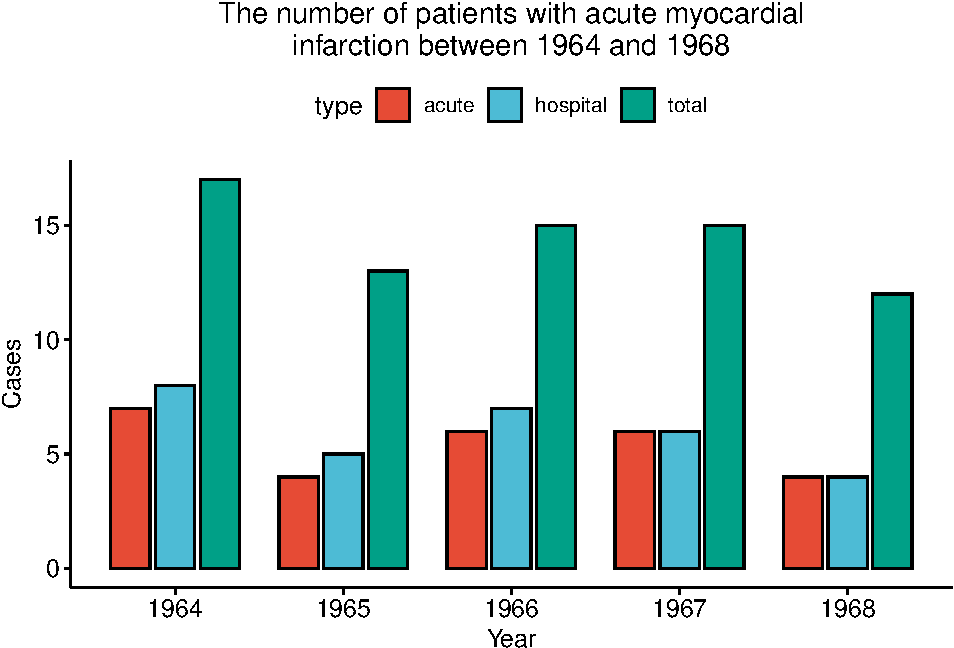
\includegraphics{Reference_solutions_files/figure-latex/unnamed-chunk-4-1.pdf}

\begin{Shaded}
\begin{Highlighting}[]
\NormalTok{data.proportion }\OtherTok{\textless{}{-}}\NormalTok{ data.number }\SpecialCharTok{\%\textgreater{}\%} 
  \FunctionTok{mutate}\NormalTok{(}\AttributeTok{hospital =}\NormalTok{ hospital}\SpecialCharTok{/}\NormalTok{total}\SpecialCharTok{*}\DecValTok{100}\NormalTok{, }\AttributeTok{acute =}\NormalTok{ acute}\SpecialCharTok{/}\NormalTok{total}\SpecialCharTok{*}\DecValTok{100}\NormalTok{) }\SpecialCharTok{\%\textgreater{}\%} 
\NormalTok{  dplyr}\SpecialCharTok{::}\FunctionTok{select}\NormalTok{(}\SpecialCharTok{!}\NormalTok{total) }\SpecialCharTok{\%\textgreater{}\%} 
  \FunctionTok{pivot\_longer}\NormalTok{(}\AttributeTok{cols =} \SpecialCharTok{!}\NormalTok{year, }\AttributeTok{names\_to =} \StringTok{\textquotesingle{}type\textquotesingle{}}\NormalTok{, }\AttributeTok{values\_to =} \StringTok{\textquotesingle{}count\textquotesingle{}}\NormalTok{)}

\FunctionTok{ggline}\NormalTok{(}\AttributeTok{data =}\NormalTok{ data.proportion, }\AttributeTok{x =} \StringTok{\textquotesingle{}year\textquotesingle{}}\NormalTok{, }\AttributeTok{y =} \StringTok{\textquotesingle{}count\textquotesingle{}}\NormalTok{, }\AttributeTok{shape =} \StringTok{\textquotesingle{}type\textquotesingle{}}\NormalTok{, }\AttributeTok{color =} \StringTok{\textquotesingle{}type\textquotesingle{}}\NormalTok{, }
       \AttributeTok{palette =} \StringTok{\textquotesingle{}npg\textquotesingle{}}\NormalTok{, }\AttributeTok{xlab =} \StringTok{\textquotesingle{}Year\textquotesingle{}}\NormalTok{, }\AttributeTok{ylab =} \StringTok{\textquotesingle{}Proportion(\%)\textquotesingle{}}\NormalTok{, }
       \AttributeTok{title =} \StringTok{"The fatality ratio of patients with acute myocardial }
\StringTok{       infarction between 1964 and 1968"} \SpecialCharTok{\%\textgreater{}\%}\NormalTok{ stringr}\SpecialCharTok{::}\FunctionTok{str\_wrap}\NormalTok{(}\AttributeTok{width =} \DecValTok{50}\NormalTok{)) }\SpecialCharTok{+} 
  \FunctionTok{theme}\NormalTok{(}\AttributeTok{plot.title =} \FunctionTok{element\_text}\NormalTok{(}\AttributeTok{hjust =}\NormalTok{ .}\DecValTok{5}\NormalTok{))}
\end{Highlighting}
\end{Shaded}

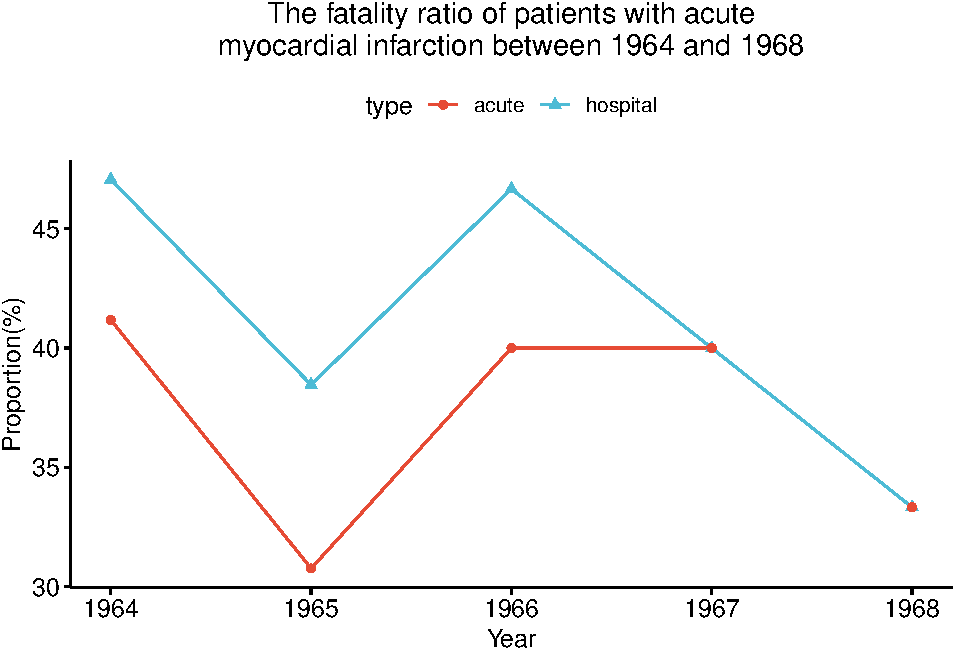
\includegraphics{Reference_solutions_files/figure-latex/unnamed-chunk-4-2.pdf}

\hypertarget{solutions-for-chapter-3}{%
\subsection{Solutions for chapter 3}\label{solutions-for-chapter-3}}

\begin{enumerate}
\def\labelenumi{\arabic{enumi}.}
\tightlist
\item
  (Page 249 3(1))
\end{enumerate}

\begin{Shaded}
\begin{Highlighting}[]
\NormalTok{conf.d }\OtherTok{\textless{}{-}} \ControlFlowTok{function}\NormalTok{(mu, sd, n) }\FunctionTok{qt}\NormalTok{(.}\DecValTok{975}\NormalTok{, }\AttributeTok{df =}\NormalTok{ n}\DecValTok{{-}1}\NormalTok{)}\SpecialCharTok{*}\FunctionTok{c}\NormalTok{(}\SpecialCharTok{{-}}\DecValTok{1}\NormalTok{, }\DecValTok{1}\NormalTok{)}\SpecialCharTok{*}\NormalTok{sd}\SpecialCharTok{/}\FunctionTok{sqrt}\NormalTok{(n) }\SpecialCharTok{+}\NormalTok{ mu}
\FunctionTok{cat}\NormalTok{(}\StringTok{\textquotesingle{}Confidence interval for 1st sample}\SpecialCharTok{\textbackslash{}n}\StringTok{\textquotesingle{}}\NormalTok{)}
\end{Highlighting}
\end{Shaded}

\begin{verbatim}
## Confidence interval for 1st sample
\end{verbatim}

\begin{Shaded}
\begin{Highlighting}[]
\FunctionTok{conf.d}\NormalTok{(}\FloatTok{6.39}\NormalTok{, }\FloatTok{2.24}\NormalTok{, }\DecValTok{20}\NormalTok{)}
\end{Highlighting}
\end{Shaded}

\begin{verbatim}
## [1] 5.341648 7.438352
\end{verbatim}

\begin{Shaded}
\begin{Highlighting}[]
\FunctionTok{cat}\NormalTok{(}\StringTok{\textquotesingle{}confidence interval for 2nd sample}\SpecialCharTok{\textbackslash{}n}\StringTok{\textquotesingle{}}\NormalTok{)}
\end{Highlighting}
\end{Shaded}

\begin{verbatim}
## confidence interval for 2nd sample
\end{verbatim}

\begin{Shaded}
\begin{Highlighting}[]
\FunctionTok{conf.d}\NormalTok{(}\FloatTok{6.45}\NormalTok{, }\FloatTok{2.51}\NormalTok{, }\DecValTok{93}\NormalTok{)}
\end{Highlighting}
\end{Shaded}

\begin{verbatim}
## [1] 5.933072 6.966928
\end{verbatim}

Sample 2 has a shorter confidence interval compared with sample 1.
Sample 1 is more reliable because of larger sample size, shorter
confidence interval.

\begin{enumerate}
\def\labelenumi{\arabic{enumi}.}
\setcounter{enumi}{1}
\tightlist
\item
  (Page 249 3(2))
\end{enumerate}

\begin{Shaded}
\begin{Highlighting}[]
\NormalTok{t.stat }\OtherTok{\textless{}{-}} \FunctionTok{sqrt}\NormalTok{(}\DecValTok{360}\NormalTok{)}\SpecialCharTok{*}\NormalTok{(}\FloatTok{4.66} \SpecialCharTok{{-}} \FloatTok{4.84}\NormalTok{)}\SpecialCharTok{/}\FloatTok{0.58}
\FunctionTok{pt}\NormalTok{(t.stat, }\AttributeTok{df =} \DecValTok{360{-}1}\NormalTok{, }\AttributeTok{lower.tail =} \ConstantTok{TRUE}\NormalTok{)}
\end{Highlighting}
\end{Shaded}

\begin{verbatim}
## [1] 4.482972e-09
\end{verbatim}

The p-value is less than 0.05, suggesting that there is significant
difference.

\textbf{Caution: this is a one-side hypothesis !}

\begin{enumerate}
\def\labelenumi{\arabic{enumi}.}
\setcounter{enumi}{2}
\tightlist
\item
  (Page 249 3(4))
\end{enumerate}

\begin{Shaded}
\begin{Highlighting}[]
\NormalTok{barx }\OtherTok{\textless{}{-}} \FunctionTok{c}\NormalTok{(}\FloatTok{11.6}\NormalTok{, }\FloatTok{6.9}\NormalTok{)}
\NormalTok{sdx }\OtherTok{\textless{}{-}} \FunctionTok{c}\NormalTok{(}\FloatTok{7.3}\NormalTok{, }\FloatTok{2.7}\NormalTok{)}
\NormalTok{varx }\OtherTok{\textless{}{-}}\NormalTok{ sdx}\SpecialCharTok{**}\DecValTok{2}
\NormalTok{n }\OtherTok{\textless{}{-}} \DecValTok{40}
\FunctionTok{cat}\NormalTok{(}\StringTok{\textquotesingle{}p{-}value for equal variance testing}\SpecialCharTok{\textbackslash{}n}\StringTok{\textquotesingle{}}\NormalTok{)}
\end{Highlighting}
\end{Shaded}

\begin{verbatim}
## p-value for equal variance testing
\end{verbatim}

\begin{Shaded}
\begin{Highlighting}[]
\FunctionTok{pf}\NormalTok{(varx[}\DecValTok{1}\NormalTok{]}\SpecialCharTok{/}\NormalTok{varx[}\DecValTok{2}\NormalTok{], }\AttributeTok{df1 =}\NormalTok{ n}\DecValTok{{-}1}\NormalTok{, }\AttributeTok{df2 =}\NormalTok{ n}\DecValTok{{-}1}\NormalTok{, }\AttributeTok{lower.tail =} \ConstantTok{FALSE}\NormalTok{)}
\end{Highlighting}
\end{Shaded}

\begin{verbatim}
## [1] 4.333099e-09
\end{verbatim}

We can't reckon that two samples have identical variance. We use
Satterthwaite approximation to test mean level, where under \(H_0\),
\(T = \frac{\bar{X} -\bar{Y}}{\sqrt{S_1^2/n_1 + S_2^2/n_2}} \approx t(m^{*})\)
with
\(m^{*} = (S_1^2/n_1 + S_2^2/n_2)^2/[\frac{1}{n_1 - 1}(S_1^2/n_1)^2 + \frac{1}{n_2 - 1}(S_2^2/n_2)^2]\).

\begin{Shaded}
\begin{Highlighting}[]
\NormalTok{m }\OtherTok{\textless{}{-}}\NormalTok{ ( (}\FunctionTok{sum}\NormalTok{(varx)}\SpecialCharTok{/}\NormalTok{n)}\SpecialCharTok{**}\DecValTok{2}\SpecialCharTok{/}\NormalTok{(}\DecValTok{1}\SpecialCharTok{/}\NormalTok{(n }\SpecialCharTok{{-}} \DecValTok{1}\NormalTok{)}\SpecialCharTok{*}\FunctionTok{sum}\NormalTok{((varx}\SpecialCharTok{/}\NormalTok{n)}\SpecialCharTok{**}\DecValTok{2}\NormalTok{)) )}\SpecialCharTok{\%\textgreater{}\%}\FunctionTok{round}\NormalTok{()}
\NormalTok{t.stat }\OtherTok{\textless{}{-}}\NormalTok{ (barx[}\DecValTok{1}\NormalTok{] }\SpecialCharTok{{-}}\NormalTok{ barx[}\DecValTok{2}\NormalTok{])}\SpecialCharTok{/}\FunctionTok{sqrt}\NormalTok{(}\FunctionTok{sum}\NormalTok{(varx}\SpecialCharTok{/}\NormalTok{n))}
\FunctionTok{cat}\NormalTok{(}\StringTok{\textquotesingle{}p{-}value is}\SpecialCharTok{\textbackslash{}n}\StringTok{\textquotesingle{}}\NormalTok{)}
\end{Highlighting}
\end{Shaded}

\begin{verbatim}
## p-value is
\end{verbatim}

\begin{Shaded}
\begin{Highlighting}[]
\DecValTok{2}\SpecialCharTok{*}\FunctionTok{pt}\NormalTok{(t.stat, }\AttributeTok{df =}\NormalTok{ m, }\AttributeTok{lower.tail =} \ConstantTok{FALSE}\NormalTok{)}
\end{Highlighting}
\end{Shaded}

\begin{verbatim}
## [1] 0.0003773703
\end{verbatim}

There is significant difference between two groups as p-value less than
0.05.

\hypertarget{solutions-for-chapter-4}{%
\subsection{Solutions for chapter 4}\label{solutions-for-chapter-4}}

\begin{enumerate}
\def\labelenumi{\arabic{enumi}.}
\tightlist
\item
  (Page 254, 3(3))
\end{enumerate}

\begin{Shaded}
\begin{Highlighting}[]
\NormalTok{p}\FloatTok{.0} \OtherTok{\textless{}{-}} \FloatTok{0.2}
\NormalTok{n}\FloatTok{.0} \OtherTok{\textless{}{-}} \DecValTok{400}
\NormalTok{x\_lower }\OtherTok{\textless{}{-}} \FunctionTok{qnorm}\NormalTok{(}\FloatTok{0.95}\NormalTok{)}\SpecialCharTok{*}\FunctionTok{sqrt}\NormalTok{(n}\FloatTok{.0}\SpecialCharTok{*}\NormalTok{p}\FloatTok{.0}\SpecialCharTok{*}\NormalTok{(}\DecValTok{1} \SpecialCharTok{{-}}\NormalTok{ p}\FloatTok{.0}\NormalTok{)) }\SpecialCharTok{+}\NormalTok{ n}\FloatTok{.0}\SpecialCharTok{*}\NormalTok{p}\FloatTok{.0}
\NormalTok{x\_lower }\SpecialCharTok{\%\textgreater{}\%} \FunctionTok{ceiling}\NormalTok{()}
\end{Highlighting}
\end{Shaded}

\begin{verbatim}
## [1] 94
\end{verbatim}

The above code uses normal approximation, while the following code
calculates exact p-value

\begin{Shaded}
\begin{Highlighting}[]
\FunctionTok{qbinom}\NormalTok{(}\FloatTok{0.95}\NormalTok{, }\DecValTok{400}\NormalTok{, }\AttributeTok{prob =} \FloatTok{0.2}\NormalTok{) }\SpecialCharTok{\%\textgreater{}\%} \FunctionTok{ceiling}\NormalTok{()}
\end{Highlighting}
\end{Shaded}

\begin{verbatim}
## [1] 93
\end{verbatim}

\textbf{Caution: it is a one-side hypothesis testing with $H_0: p > 0.2$}

\begin{enumerate}
\def\labelenumi{\arabic{enumi}.}
\setcounter{enumi}{1}
\tightlist
\item
  (Page 254, 3(1))
\end{enumerate}

\begin{Shaded}
\begin{Highlighting}[]
\FunctionTok{poisson.test}\NormalTok{(}\DecValTok{225}\NormalTok{, }\AttributeTok{r =} \DecValTok{100}\SpecialCharTok{*}\DecValTok{2}\NormalTok{, }\AttributeTok{alternative =} \StringTok{\textquotesingle{}greater\textquotesingle{}}\NormalTok{)}
\end{Highlighting}
\end{Shaded}

\begin{verbatim}
## 
##  Exact Poisson test
## 
## data:  225 time base: 1
## number of events = 225, time base = 1, p-value = 0.04361
## alternative hypothesis: true event rate is greater than 200
## 95 percent confidence interval:
##  200.9087      Inf
## sample estimates:
## event rate 
##        225
\end{verbatim}

With a p-value less than 0.05, we reject the null hypothesis and
conclude that the water is \emph{unqualified}.

\textbf{Caution: sum of two independent poisson distribution does also follow a poisson distribution; it's also a one-side hypothesis testing}

\begin{enumerate}
\def\labelenumi{\arabic{enumi}.}
\setcounter{enumi}{2}
\tightlist
\item
  (Page 256, 3(1))
\end{enumerate}

\begin{Shaded}
\begin{Highlighting}[]
\NormalTok{data.drug }\OtherTok{\textless{}{-}} \FunctionTok{matrix}\NormalTok{(}\FunctionTok{c}\NormalTok{(}\DecValTok{28}\NormalTok{, }\DecValTok{18}\NormalTok{, }\DecValTok{10}\NormalTok{, }\DecValTok{9}\NormalTok{, }\DecValTok{20}\NormalTok{, }\DecValTok{24}\NormalTok{), }\AttributeTok{nrow =} \DecValTok{3}\NormalTok{)}
\FunctionTok{chisq.test}\NormalTok{(data.drug, }\AttributeTok{correct =} \ConstantTok{FALSE}\NormalTok{)}
\end{Highlighting}
\end{Shaded}

\begin{verbatim}
## 
##  Pearson's Chi-squared test
## 
## data:  data.drug
## X-squared = 15.556, df = 2, p-value = 0.0004189
\end{verbatim}

Significant difference.

\begin{enumerate}
\def\labelenumi{\arabic{enumi}.}
\setcounter{enumi}{3}
\tightlist
\item
  (Page 256, 3(4))
\end{enumerate}

\begin{Shaded}
\begin{Highlighting}[]
\NormalTok{data.co }\OtherTok{\textless{}{-}} \FunctionTok{matrix}\NormalTok{(}\FunctionTok{c}\NormalTok{(}\DecValTok{120}\SpecialCharTok{*}\FloatTok{0.35}\NormalTok{, }\DecValTok{120}\SpecialCharTok{*}\NormalTok{(}\FloatTok{0.6} \SpecialCharTok{{-}} \FloatTok{0.35}\NormalTok{), }
                    \DecValTok{120}\SpecialCharTok{*}\NormalTok{(}\FloatTok{0.5} \SpecialCharTok{{-}} \FloatTok{0.35}\NormalTok{), }\DecValTok{120}\SpecialCharTok{*}\NormalTok{(}\DecValTok{1} \SpecialCharTok{{-}} \FloatTok{0.35} \SpecialCharTok{{-}} \FloatTok{0.25} \SpecialCharTok{{-}} \FloatTok{0.15}\NormalTok{)), }
                  \AttributeTok{nrow =} \DecValTok{2}\NormalTok{)}
\FunctionTok{mcnemar.test}\NormalTok{(data.co)}
\end{Highlighting}
\end{Shaded}

\begin{verbatim}
## 
##  McNemar's Chi-squared test with continuity correction
## 
## data:  data.co
## McNemar's chi-squared = 2.5208, df = 1, p-value = 0.1124
\end{verbatim}

No significant differences.

\hypertarget{solutions-for-chapter-5}{%
\subsection{Solutions for chapter 5}\label{solutions-for-chapter-5}}

\begin{enumerate}
\def\labelenumi{\arabic{enumi}.}
\tightlist
\item
  (Page 258, 1)
\end{enumerate}

\begin{Shaded}
\begin{Highlighting}[]
\NormalTok{data.thyroid }\OtherTok{\textless{}{-}} \FunctionTok{data.frame}\NormalTok{(}\AttributeTok{group =} \FunctionTok{c}\NormalTok{(}\FunctionTok{rep}\NormalTok{(}\StringTok{\textquotesingle{}high\textquotesingle{}}\NormalTok{, }\DecValTok{9}\NormalTok{), }\FunctionTok{rep}\NormalTok{(}\StringTok{\textquotesingle{}mid\textquotesingle{}}\NormalTok{, }\DecValTok{8}\NormalTok{), }\FunctionTok{rep}\NormalTok{(}\StringTok{\textquotesingle{}low\textquotesingle{}}\NormalTok{, }\DecValTok{7}\NormalTok{)) }\SpecialCharTok{\%\textgreater{}\%} \FunctionTok{factor}\NormalTok{(), }
                           \AttributeTok{thyroid =} \FunctionTok{c}\NormalTok{(}\DecValTok{34}\NormalTok{, }\DecValTok{45}\NormalTok{, }\DecValTok{49}\NormalTok{, }\DecValTok{55}\NormalTok{, }\DecValTok{58}\NormalTok{, }\DecValTok{59}\NormalTok{, }\DecValTok{60}\NormalTok{, }\DecValTok{72}\NormalTok{, }\DecValTok{86}\NormalTok{, }\DecValTok{8}\NormalTok{, }\DecValTok{25}\NormalTok{, }\DecValTok{36}\NormalTok{, }
                                       \DecValTok{40}\NormalTok{, }\DecValTok{42}\NormalTok{, }\DecValTok{53}\NormalTok{, }\DecValTok{65}\NormalTok{, }\DecValTok{74}\NormalTok{, }\DecValTok{5}\NormalTok{, }\DecValTok{8}\NormalTok{, }\DecValTok{18}\NormalTok{, }\DecValTok{32}\NormalTok{, }\DecValTok{45}\NormalTok{, }\DecValTok{47}\NormalTok{, }\DecValTok{65}\NormalTok{))}

\FunctionTok{bartlett.test}\NormalTok{(thyroid }\SpecialCharTok{\textasciitilde{}}\NormalTok{ group, }\AttributeTok{data =}\NormalTok{ data.thyroid)}
\end{Highlighting}
\end{Shaded}

\begin{verbatim}
## 
##  Bartlett test of homogeneity of variances
## 
## data:  thyroid by group
## Bartlett's K-squared = 1.1653, df = 2, p-value = 0.5584
\end{verbatim}

\begin{Shaded}
\begin{Highlighting}[]
\NormalTok{fit.thyroid }\OtherTok{\textless{}{-}} \FunctionTok{aov}\NormalTok{(thyroid }\SpecialCharTok{\textasciitilde{}}\NormalTok{ group, }\AttributeTok{data =}\NormalTok{ data.thyroid)}
\FunctionTok{summary}\NormalTok{(fit.thyroid)}
\end{Highlighting}
\end{Shaded}

\begin{verbatim}
##             Df Sum Sq Mean Sq F value Pr(>F)  
## group        2   2744  1372.1   3.623 0.0445 *
## Residuals   21   7953   378.7                 
## ---
## Signif. codes:  0 '***' 0.001 '**' 0.01 '*' 0.05 '.' 0.1 ' ' 1
\end{verbatim}

\begin{Shaded}
\begin{Highlighting}[]
\FunctionTok{cat}\NormalTok{(}\StringTok{"No difference in variance. Significant difference in average }
\StringTok{    level for each group."}\NormalTok{)}
\end{Highlighting}
\end{Shaded}

\begin{verbatim}
## No difference in variance. Significant difference in average 
##     level for each group.
\end{verbatim}

\begin{enumerate}
\def\labelenumi{\arabic{enumi}.}
\setcounter{enumi}{1}
\tightlist
\item
  (Page 258, 2)
\end{enumerate}

\begin{Shaded}
\begin{Highlighting}[]
\NormalTok{data.rat }\OtherTok{\textless{}{-}} \FunctionTok{data.frame}\NormalTok{(}\AttributeTok{type =} \FunctionTok{rep}\NormalTok{(}\FunctionTok{c}\NormalTok{(}\StringTok{\textquotesingle{}A\textquotesingle{}}\NormalTok{, }\StringTok{\textquotesingle{}B\textquotesingle{}}\NormalTok{, }\StringTok{\textquotesingle{}C\textquotesingle{}}\NormalTok{), }\AttributeTok{each =} \DecValTok{5}\NormalTok{) }\SpecialCharTok{\%\textgreater{}\%} \FunctionTok{factor}\NormalTok{(), }
                       \AttributeTok{group =} \FunctionTok{rep}\NormalTok{(}\DecValTok{1}\SpecialCharTok{:}\DecValTok{5}\NormalTok{, }\DecValTok{3}\NormalTok{) }\SpecialCharTok{\%\textgreater{}\%} \FunctionTok{factor}\NormalTok{(), }
                       \AttributeTok{hours =} \FunctionTok{c}\NormalTok{(}\FloatTok{1.16}\NormalTok{, }\FloatTok{2.11}\NormalTok{, }\FloatTok{1.82}\NormalTok{, }\FloatTok{1.41}\NormalTok{, }\FloatTok{0.51}\NormalTok{, }\FloatTok{1.30}\NormalTok{, }\FloatTok{3.28}\NormalTok{, }\FloatTok{4.98}\NormalTok{, }
                                 \FloatTok{2.59}\NormalTok{, }\FloatTok{0.59}\NormalTok{, }\FloatTok{3.36}\NormalTok{, }\FloatTok{5.28}\NormalTok{, }\FloatTok{4.81}\NormalTok{, }\FloatTok{2.04}\NormalTok{, }\FloatTok{5.05}\NormalTok{))}

\NormalTok{fit.rat }\OtherTok{\textless{}{-}} \FunctionTok{aov}\NormalTok{(hours }\SpecialCharTok{\textasciitilde{}}\NormalTok{ type }\SpecialCharTok{+}\NormalTok{ group, }\AttributeTok{data=}\NormalTok{ data.rat)}
\FunctionTok{summary}\NormalTok{(fit.rat)}
\end{Highlighting}
\end{Shaded}

\begin{verbatim}
##             Df Sum Sq Mean Sq F value Pr(>F)  
## type         2  18.45   9.224   7.204 0.0162 *
## group        4  10.72   2.680   2.093 0.1736  
## Residuals    8  10.24   1.280                 
## ---
## Signif. codes:  0 '***' 0.001 '**' 0.01 '*' 0.05 '.' 0.1 ' ' 1
\end{verbatim}

\begin{Shaded}
\begin{Highlighting}[]
\FunctionTok{cat}\NormalTok{(}\StringTok{"No significant difference for each group but there is significant }
\StringTok{    difference for various types of drug. "}\NormalTok{)}
\end{Highlighting}
\end{Shaded}

\begin{verbatim}
## No significant difference for each group but there is significant 
##     difference for various types of drug.
\end{verbatim}

\begin{enumerate}
\def\labelenumi{\arabic{enumi}.}
\setcounter{enumi}{2}
\tightlist
\item
  (Page 258, 3)
\end{enumerate}

\begin{Shaded}
\begin{Highlighting}[]
\NormalTok{dummy }\OtherTok{\textless{}{-}} \FunctionTok{data.frame}\NormalTok{(}\AttributeTok{before =} \FunctionTok{c}\NormalTok{(}\DecValTok{4}\NormalTok{, }\FloatTok{3.5}\NormalTok{, }\FloatTok{3.2}\NormalTok{, }\FloatTok{3.2}\NormalTok{, }\FloatTok{3.3}\NormalTok{, }\FloatTok{3.4}\NormalTok{, }\FloatTok{2.7}\NormalTok{, }\FloatTok{4.8}\NormalTok{, }\FloatTok{4.5}\NormalTok{, }\FloatTok{3.8}\NormalTok{), }
                    \AttributeTok{after =} \FunctionTok{c}\NormalTok{(}\FloatTok{5.4}\NormalTok{, }\FloatTok{4.7}\NormalTok{, }\FloatTok{5.2}\NormalTok{, }\FloatTok{4.8}\NormalTok{, }\FloatTok{4.6}\NormalTok{, }\FloatTok{4.9}\NormalTok{, }\FloatTok{3.8}\NormalTok{, }\FloatTok{6.1}\NormalTok{, }\FloatTok{5.9}\NormalTok{, }\FloatTok{4.9}\NormalTok{))}
\NormalTok{dummy\_diff }\OtherTok{\textless{}{-}} \FunctionTok{with}\NormalTok{(dummy, after }\SpecialCharTok{{-}}\NormalTok{ before)}

\NormalTok{pills }\OtherTok{\textless{}{-}} \FunctionTok{data.frame}\NormalTok{(}\AttributeTok{before =} \FunctionTok{c}\NormalTok{(}\FloatTok{3.5}\NormalTok{, }\FloatTok{3.3}\NormalTok{, }\FloatTok{3.2}\NormalTok{, }\FloatTok{4.5}\NormalTok{, }\FloatTok{4.3}\NormalTok{, }\FloatTok{3.2}\NormalTok{, }\FloatTok{4.2}\NormalTok{, }\FloatTok{5.}\NormalTok{, }\FloatTok{4.3}\NormalTok{, }\FloatTok{3.6}\NormalTok{), }
                    \AttributeTok{after =} \FunctionTok{c}\NormalTok{(}\FloatTok{4.7}\NormalTok{, }\FloatTok{4.4}\NormalTok{, }\FloatTok{4.}\NormalTok{, }\FloatTok{5.2}\NormalTok{, }\FloatTok{5.}\NormalTok{, }\FloatTok{4.3}\NormalTok{, }\FloatTok{5.1}\NormalTok{, }\FloatTok{6.5}\NormalTok{, }\FloatTok{4.}\NormalTok{, }\FloatTok{4.7}\NormalTok{))}
\NormalTok{pills\_diff }\OtherTok{\textless{}{-}} \FunctionTok{with}\NormalTok{(pills, after }\SpecialCharTok{{-}}\NormalTok{ before)}

\NormalTok{dt.combined }\OtherTok{\textless{}{-}} \FunctionTok{data.frame}\NormalTok{(}\AttributeTok{dummy =}\NormalTok{ dummy\_diff, }\AttributeTok{pills =}\NormalTok{ pills\_diff) }\SpecialCharTok{\%\textgreater{}\%}
    \FunctionTok{pivot\_longer}\NormalTok{(}\AttributeTok{cols =} \FunctionTok{everything}\NormalTok{(), }\AttributeTok{names\_to =} \StringTok{"group"}\NormalTok{, }\AttributeTok{values\_to =} \StringTok{"hours"}\NormalTok{) }\SpecialCharTok{\%\textgreater{}\%}
    \FunctionTok{mutate}\NormalTok{(}\AttributeTok{group =} \FunctionTok{factor}\NormalTok{(group))}
\FunctionTok{bartlett.test}\NormalTok{(hours }\SpecialCharTok{\textasciitilde{}}\NormalTok{ group, }\AttributeTok{data =}\NormalTok{ dt.combined)}
\end{Highlighting}
\end{Shaded}

\begin{verbatim}
## 
##  Bartlett test of homogeneity of variances
## 
## data:  hours by group
## Bartlett's K-squared = 2.7758, df = 1, p-value = 0.0957
\end{verbatim}

\begin{Shaded}
\begin{Highlighting}[]
\FunctionTok{t.test}\NormalTok{(dummy\_diff, pills\_diff, }\AttributeTok{var.equal =} \ConstantTok{TRUE}\NormalTok{)}
\end{Highlighting}
\end{Shaded}

\begin{verbatim}
## 
##  Two Sample t-test
## 
## data:  dummy_diff and pills_diff
## t = 2.9203, df = 18, p-value = 0.009137
## alternative hypothesis: true difference in means is not equal to 0
## 95 percent confidence interval:
##  0.1430897 0.8769103
## sample estimates:
## mean of x mean of y 
##      1.39      0.88
\end{verbatim}

\begin{Shaded}
\begin{Highlighting}[]
\FunctionTok{cat}\NormalTok{(}\StringTok{"No difference in variance. By t{-}test we can conclude that there is significant }
\StringTok{    different between the effect of pills and that of placebo."}\NormalTok{)}
\end{Highlighting}
\end{Shaded}

\begin{verbatim}
## No difference in variance. By t-test we can conclude that there is significant 
##     different between the effect of pills and that of placebo.
\end{verbatim}

\hypertarget{solutions-for-chapter-6}{%
\subsection{Solutions for chapter 6}\label{solutions-for-chapter-6}}

\begin{enumerate}
\def\labelenumi{\arabic{enumi}.}
\tightlist
\item
  (Page 260 1)
\end{enumerate}

\begin{enumerate}
\def\labelenumi{(\arabic{enumi})}
\tightlist
\item
\end{enumerate}

\begin{Shaded}
\begin{Highlighting}[]
\NormalTok{data.cstu }\OtherTok{\textless{}{-}} \FunctionTok{data.frame}\NormalTok{(}\AttributeTok{height=} \FunctionTok{c}\NormalTok{(}\DecValTok{170}\NormalTok{, }\DecValTok{173}\NormalTok{, }\DecValTok{160}\NormalTok{, }\DecValTok{155}\NormalTok{, }\DecValTok{173}\NormalTok{, }\DecValTok{188}\NormalTok{, }\DecValTok{178}\NormalTok{, }\DecValTok{183}\NormalTok{, }\DecValTok{180}\NormalTok{, }\DecValTok{165}\NormalTok{), }
                        \AttributeTok{frontarm =} \FunctionTok{c}\NormalTok{(}\DecValTok{45}\NormalTok{, }\DecValTok{42}\NormalTok{, }\DecValTok{44}\NormalTok{, }\DecValTok{41}\NormalTok{, }\DecValTok{47}\NormalTok{, }\DecValTok{50}\NormalTok{, }\DecValTok{47}\NormalTok{, }\DecValTok{46}\NormalTok{, }\DecValTok{49}\NormalTok{, }\DecValTok{43}\NormalTok{))}
\FunctionTok{ggscatter}\NormalTok{(}\AttributeTok{data =}\NormalTok{ data.cstu, }\AttributeTok{x =} \StringTok{\textquotesingle{}height\textquotesingle{}}\NormalTok{, }\AttributeTok{y =} \StringTok{\textquotesingle{}frontarm\textquotesingle{}}\NormalTok{, }\AttributeTok{palette =} \StringTok{\textquotesingle{}npg\textquotesingle{}}\NormalTok{, }
          \AttributeTok{shape =} \DecValTok{3}\NormalTok{, }\AttributeTok{title =} \StringTok{\textquotesingle{}Scatterplot between Height and Front Arm Length\textquotesingle{}}\NormalTok{, }
          \AttributeTok{add =} \StringTok{\textquotesingle{}reg.line\textquotesingle{}}\NormalTok{)}
\end{Highlighting}
\end{Shaded}

\begin{verbatim}
## `geom_smooth()` using formula 'y ~ x'
\end{verbatim}

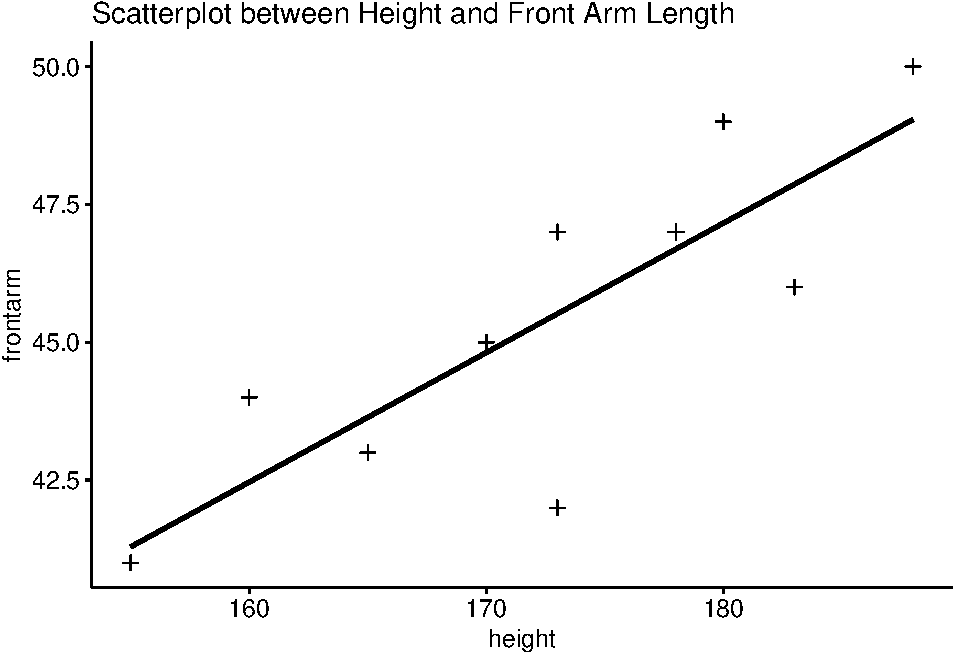
\includegraphics{Reference_solutions_files/figure-latex/unnamed-chunk-17-1.pdf}

\begin{Shaded}
\begin{Highlighting}[]
\FunctionTok{with}\NormalTok{(data.cstu, }\FunctionTok{cor}\NormalTok{(height, frontarm))}
\end{Highlighting}
\end{Shaded}

\begin{verbatim}
## [1] 0.8227162
\end{verbatim}

\begin{Shaded}
\begin{Highlighting}[]
\FunctionTok{with}\NormalTok{(data.cstu, }\FunctionTok{cor.test}\NormalTok{(height, frontarm))}
\end{Highlighting}
\end{Shaded}

\begin{verbatim}
## 
##  Pearson's product-moment correlation
## 
## data:  height and frontarm
## t = 4.0936, df = 8, p-value = 0.003468
## alternative hypothesis: true correlation is not equal to 0
## 95 percent confidence interval:
##  0.4006045 0.9567450
## sample estimates:
##       cor 
## 0.8227162
\end{verbatim}

Figure shows they are jointly normal distributed. We use Pearson's test
for correlation (\(P < 0.01\)). The results show that Height and Length
of front arm are correlated, with Pearson's correlation coefficient as
0.82.

\begin{enumerate}
\def\labelenumi{(\arabic{enumi})}
\setcounter{enumi}{1}
\tightlist
\item
\end{enumerate}

\begin{Shaded}
\begin{Highlighting}[]
\NormalTok{mod.xy }\OtherTok{\textless{}{-}} \FunctionTok{lm}\NormalTok{(height }\SpecialCharTok{\textasciitilde{}}\NormalTok{ frontarm, }\AttributeTok{data =}\NormalTok{ data.cstu)}
\FunctionTok{summary}\NormalTok{(mod.xy)}
\end{Highlighting}
\end{Shaded}

\begin{verbatim}
## 
## Call:
## lm(formula = height ~ frontarm, data = data.cstu)
## 
## Residuals:
##     Min      1Q  Median      3Q     Max 
## -8.4643 -3.8036 -0.9643  1.9018 10.3010 
## 
## Coefficients:
##             Estimate Std. Error t value Pr(>|t|)   
## (Intercept)  41.6276    32.0311   1.300  0.22993   
## frontarm      2.8827     0.7042   4.094  0.00347 **
## ---
## Signif. codes:  0 '***' 0.001 '**' 0.01 '*' 0.05 '.' 0.1 ' ' 1
## 
## Residual standard error: 6.235 on 8 degrees of freedom
## Multiple R-squared:  0.6769, Adjusted R-squared:  0.6365 
## F-statistic: 16.76 on 1 and 8 DF,  p-value: 0.003468
\end{verbatim}

\begin{Shaded}
\begin{Highlighting}[]
\FunctionTok{residualPlot}\NormalTok{(mod.xy, }\AttributeTok{id =} \ConstantTok{TRUE}\NormalTok{)}
\end{Highlighting}
\end{Shaded}

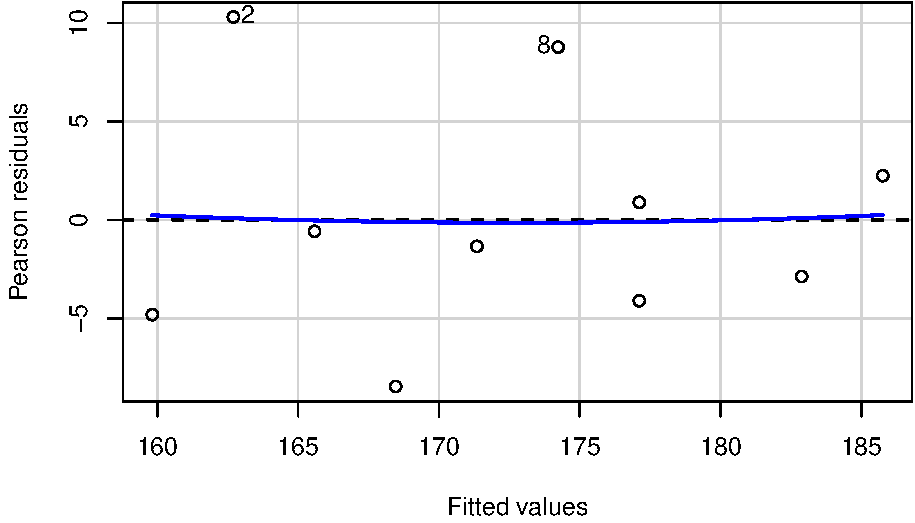
\includegraphics{Reference_solutions_files/figure-latex/unnamed-chunk-18-1.pdf}

\begin{Shaded}
\begin{Highlighting}[]
\CommentTok{\# aov(mod.xy)}
\end{Highlighting}
\end{Shaded}

The residual plot shows the residuals follow the linear assumption, and
the estimated coefficient is significantly different with 0.

\begin{Shaded}
\begin{Highlighting}[]
\NormalTok{mod.yx }\OtherTok{\textless{}{-}} \FunctionTok{lm}\NormalTok{(frontarm }\SpecialCharTok{\textasciitilde{}}\NormalTok{ height, }\AttributeTok{data =}\NormalTok{ data.cstu)}
\FunctionTok{summary}\NormalTok{(mod.yx)}
\end{Highlighting}
\end{Shaded}

\begin{verbatim}
## 
## Call:
## lm(formula = frontarm ~ height, data = data.cstu)
## 
## Residuals:
##     Min      1Q  Median      3Q     Max 
## -3.5174 -0.5519  0.2478  1.3521  1.8390 
## 
## Coefficients:
##             Estimate Std. Error t value Pr(>|t|)   
## (Intercept)  4.89610    9.91053   0.494  0.63456   
## height       0.23481    0.05736   4.094  0.00347 **
## ---
## Signif. codes:  0 '***' 0.001 '**' 0.01 '*' 0.05 '.' 0.1 ' ' 1
## 
## Residual standard error: 1.78 on 8 degrees of freedom
## Multiple R-squared:  0.6769, Adjusted R-squared:  0.6365 
## F-statistic: 16.76 on 1 and 8 DF,  p-value: 0.003468
\end{verbatim}

\begin{Shaded}
\begin{Highlighting}[]
\FunctionTok{residualPlot}\NormalTok{(mod.yx)}
\end{Highlighting}
\end{Shaded}

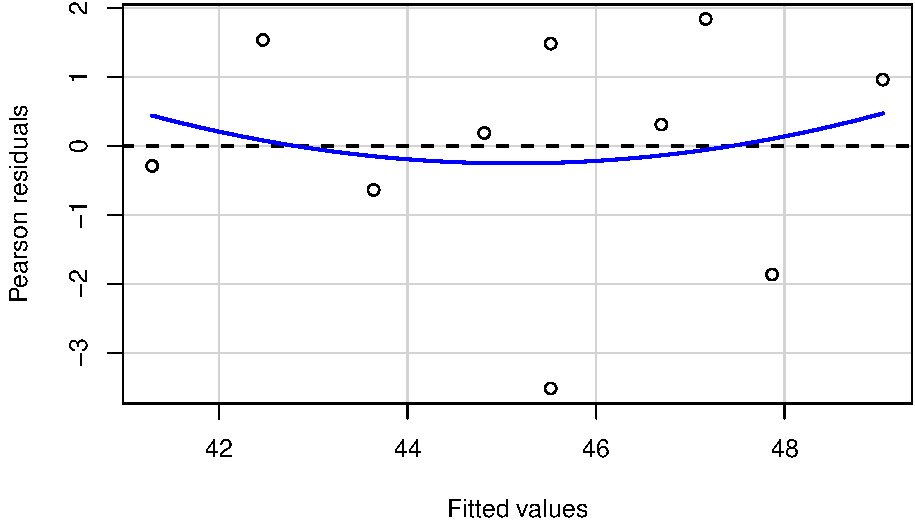
\includegraphics{Reference_solutions_files/figure-latex/unnamed-chunk-19-1.pdf}

\begin{Shaded}
\begin{Highlighting}[]
\CommentTok{\# aov(mod.yx)}
\end{Highlighting}
\end{Shaded}

The residual plot shows the residuals don't follow linear assumption, we
should make transformation to variables.

\begin{enumerate}
\def\labelenumi{\arabic{enumi}.}
\setcounter{enumi}{1}
\tightlist
\item
  (Page 260 3(1))
\end{enumerate}

Omitted.

\newpage

\hypertarget{remarks}{%
\section{Remarks}\label{remarks}}

Here lists several notes that might be forgotten

\hypertarget{chapter-2-numerical-variables-categorical-variables-and-corresponding-descriptive-tables-and-figures}{%
\subsection{chapter 2: Numerical variables, categorical variables and
corresponding descriptive tables and
figures}\label{chapter-2-numerical-variables-categorical-variables-and-corresponding-descriptive-tables-and-figures}}

\begin{itemize}
\tightlist
\item
  CV(coefficient variation) is the ratio of sample standard deviation
  with sample mean (\(\frac{S}{\bar{X}}\times 100\%\))
\item
  To test the normality of data, use \texttt{qqnorm(x);\ qqline(x)} for
  figuring and \texttt{shapiro.test(x)} for numerical testing
\item
  When comparing two groups of different total numbers, please
  standardize them implicitly(SMR) or explicitly
\item
  Ubiquitous statistical figures include
  \textbf{barplot, pie, lines, hist, stem and boxplot, .etc}
\item
  Statistical figures with standard errors can be plotted with
  \texttt{arrows(x0\ =\ x,\ y0\ =\ y\ -\ sd,\ x1\ =\ x,\ y1\ =\ y\ \ +sd,\ angle\ =\ ,\ length\ =\ )}
\end{itemize}

\hypertarget{chapter-3-estimation-and-hypothesis-testing-for-overall-mean}{%
\subsection{chapter 3: Estimation and hypothesis testing for overall
mean}\label{chapter-3-estimation-and-hypothesis-testing-for-overall-mean}}

\begin{itemize}
\tightlist
\item
  Standard error: the standard deviation of sample mean, denoted by
  \(\sigma_{\bar{X}} = \frac{\sigma}{\sqrt{n}}\)
\item
  Estimation: moment estimation and maximizing the likelihood(mle)
\item
  General methods for deriving interval estimation: (1) find out a
  random variable \(f(X_1, \dots, X_n, \theta)\) with a given
  distribution having nothing with \(\theta\), denoted as \(F(x)\); (2)
  find out \(a, b\) so that \(F(b) - F(a) = 1- \alpha\); (3) transform
  \(f(X_1, \dots, X_n, \theta) \in (a, b]\) into the form of \(\theta\)
  that \(\theta \in (\theta_1, \theta_2)\)
\item
  Summarize the basic approaches of interval estimation: (1) if
  \(\sigma\) is given, then \(z-\)distribution; (2) if \(\sigma\) is not
  given, then \(t-\)distribution
\item
  Hypothesis testing. For variance testing, (1)
  \(H_0: \sigma = \sigma_0\), use \(\chi^2-\)test; (2)
  \(H_0: \sigma_1^2 = \sigma_2^2\), use \(F-\)test. For sample mean,
  similar with interval estimation in single sample testing. For two
  samples, (1) paired, use \texttt{t.test(x,\ y,\ paired\ =\ TRUE)}; (2)
  assuming equal variance, use
  \texttt{t.test(x,\ y,\ var.equal\ =\ TRUE)}; else use
  \texttt{t.test(x,\ y,\ var.equal\ =\ FALSE)}
\item
  Understand two type errors. (Under fixed type 1 error, we can reduce
  type 2 error by putting on samples)
\item
  Non-parametric testing for sample median: Rank-sum test, use
  \texttt{wilcox.test(x,\ y)}.
\end{itemize}

\hypertarget{chapter-4-binomial-poisson-distribution-and-hypothesis-testing-for-categorical-variables}{%
\subsection{chapter 4: Binomial, Poisson distribution and hypothesis
testing for categorical
variables}\label{chapter-4-binomial-poisson-distribution-and-hypothesis-testing-for-categorical-variables}}

\begin{itemize}
\tightlist
\item
  Hypothesis testing for poisson distributed samples: (1) single sample,
  use normal approximation
  \(\frac{X - \lambda_0}{\sqrt{\lambda_0}} \sim N(0, 1)\); (2) two
  samples, under \(H_0: \lambda_1 = \lambda_2\) if
  \(X_1 \sim \text{Pois}(n_1\lambda_1)\) and
  \(X_2 \sim \text{Pois}(n_2\lambda_2)\), then
  \((X_1/n_1 - X_2/n_2)/\sqrt{X_1/n_1^2 + X_2/n_2^2}\approx N(0, 1)\)
\item
  In following situations \(\chi^2-\)test works, (1) Goodness-of-fit,
  \texttt{chisq.test(x,\ p\ =\ )}; (2) test for non-correlation,
  \texttt{chisq.test(xmatrix,\ correct\ =\ )}; or u can use fisher exact
  testing, \texttt{fisher.test(data,\ alternative\ \ =)}; (3) paired
  design, \texttt{mcnemar.test(data)}
\end{itemize}

\hypertarget{chapter-5-analysis-of-variance}{%
\subsection{chapter 5: Analysis of
variance}\label{chapter-5-analysis-of-variance}}

\begin{itemize}
\tightlist
\item
  Major goal: compare the mean between two or more groups
\item
  Basic assumptions: (1) within each group, samples follow normal
  distribution with identical variance (2) independence
\item
  R code for anova: (1) testing the homoscedasticity,
  \texttt{barlett.test(score\ \textasciitilde{}\ group,\ data\ =\ )};
  (2) anova,
  \texttt{score.aov\ =\ aov(score\ \textasciitilde{}\ group,\ data\ =\ );\ summary(score.aov)};
  (3) randomized-block design,
  \texttt{aov(score\ \textasciitilde{}\ blocknum\ +\ group,\ data\ =\ )\ \%\textgreater{}\%\ summary()};
  (4) analysis of covariance,
  \texttt{fit\ \textless{}-\ aov(score\ \textasciitilde{}\ age\ +\ group,\ data\ =\ );\ summary(fit)};
  to show group effects,
  \texttt{library(effects);\ effect("group",\ fit)}; to pairwise
  compare,
  \texttt{library(multcomp);\ res.vsl\ =\ glht(fit,\ linfct\ =\ mcp(group\ =\ c("a\ -b\ =\ 0",\ "b\ -\ c\ =\ 0",\ "a\ -\ c\ =\ 0")));\ summary(res.vsl,\ test\ =\ adjusted("bonferroni"))}
\item
  For a pairwise comparison, we can use a post hoc test with adjust
  p-value,
  \texttt{pairwise.t.test(group,\ score,\ p.adjust.method\ =\ "holm")}
\end{itemize}

\hypertarget{chapter-6-regression-analysis}{%
\subsection{chapter 6: regression
analysis}\label{chapter-6-regression-analysis}}

\begin{itemize}
\tightlist
\item
  Compute the correlations. (1) when data follows joint normal
  distribution, then use pearson correlation
  \texttt{cor(x,\ y,\ method\ =\ \textquotesingle{}pearson\textquotesingle{});\ cor.test(..)};
  (draw figures to verify the joint normality first) (2) when data does
  not follow normal distribution, then use spearman's correlation,
  \texttt{cor(x,\ y,\ method\ =\ "spearman")}
\item
  Statistical inference in linear regression model. (1) t-test for
  coefficients, \texttt{confint(model,\ level\ =\ .95)}; (2) for fitting
  and prediction, the interval estimations are not identical,
  \texttt{predict(model,\ newdata\ =\ data.frame(var\ =\ ),\ interval\ =\ c(\textquotesingle{}prediction\textquotesingle{},\ \textquotesingle{}confidence\textquotesingle{}),\ level\ =\ .95)}.
\item
  Life table (Omitted)
\end{itemize}

\hypertarget{suggestions-for-advanced-r-or-statistics}{%
\section{Suggestions for advanced R or
statistics}\label{suggestions-for-advanced-r-or-statistics}}

For more advanced usages of R code, you can refer to

\begin{itemize}
\tightlist
\item
  A tutorial written by Dongfeng Li, Peking University, attached link:
  \url{https://www.math.pku.edu.cn/teachers/lidf/docs/Rbook/html/_Rbook/index.html}
\item
  R Cookbook, 2nd Edition
\item
  R Graphics Cookbook, 2nd Edition (for making figures)
\end{itemize}

To obtain more knowledge on statistics, u are welcomed to take the
course hosted by Dr.~Jia on next semester, namely \emph{Statistical
modeling} !

\bibliographystyle{unsrt}
\bibliography{references.bib}


\end{document}
